\chapter{Introduzione}
\label{chapter:introduction}
Questo lavoro ha come obiettivo l'analisi di reti metaboliche:
cercheremo di astrarre i processi fisici che avvengono all'interno
delle cellule di organismi, utilizzando la struttura astratta grafo in
modo da poter ragionare su quest'ultimo utilizzando algoritmi ben noti
della teoria dei grafi. In particolare indagheremo la relazione di
connessione forte, ricercando le componenti fortemente connesse.
\\\\
In questo capitolo si definisce cosa sono le reti metaboliche, il
motivo per cui vengono studiate, come formulare un modello astratto
che descriva una rete, quali sono i risultati gi\`a noti che
condividono alcuni aspetti di questo lavoro e quali sono gli obiettivi
che vogliamo raggiungere.

% Numerosi sistemi biologici possono essere modellati con il concetto
% astratto di grafo. Studiare la struttura e la topologia di
% quest'astrazione non fornisce solo una descrizione dei complessi
% comportamenti del sistema in oggetto ma, pu\`o essere di grande
% utilit\`a per capire le funzionalit\`a del sistema e le sue dinamiche.

% Inoltre attraverso questo processo di astrazione, \`e possibile
% studiare quali relazioni possono intercorrere tra il sistema e il
% contesto che lo ospita. Lo studio di queste relazioni pu\`o portare a
% fare delle stime riguardo la potenzialit\`a del sistema di
% ``comunicare'' con il contesto.

% Le idee che abbiamo espresso sono alla base del concetto di
% \emph{storia} che avremo modo di studiare meglio nel Capitolo
% \ref{chapter:theoretical-background}.  

\section{Enzimi, cammini e reti metaboliche}

Prima di dare la definizione di \emph{rete metabolica} introduciamo i
concetti di cammino metabolico, enzima e da cosa \`e caratterizzata
una reazione chimica.

Un \emph{cammino metabolico} \`e una sequenza di reazioni chimiche che
si verificano all'interno di una cellula. Dal punto di vista
matematico, possiamo vedere un cammino metabolico come una sequenza di
funzioni, dette reazioni, che, avendo in input un insieme di molecole,
esegue delle trasformazioni su queste e produce come output il
risultato delle trasformazioni svolte, sotto forma di insieme di
molecole. Questo output pu\`o essere utilizzato come input per la
funzione successiva, concatenando quanto si voglia le trasformazioni.

Ogni reazione chimica \`e regolata da alcuni \emph{enzimi}. Un
\emph{enzima} \`e una proteina che gestisce la frequenza e la
velocit\`a di una reazione chimica. Le molecole a cui si applica la
reazione vengono identificate con il termine \emph{substrato} (o
\emph{reagenti}), mentre le molecole output della reazione vengono
identificate con il termine \emph{prodotti}.  Durante l'esecuzione di
una reazione chimica, ogni enzima agisce da \emph{catalizzatore},
ovvero non viene consumato nella reazione e, quindi, pu\`o partecipare
in pi\`u di una reazione.

L'insieme di enzimi ``guida'' e determina l'insieme di cammini
metabolici che possono occorrere nella cellula, in quanto una reazione
chimica su un substrato pu\`o avvenire se e solo se lo strato attivo
del substrato \`e complementare allo strato attivo dell'enzima.
\\\\
Adesso possiamo definire una \emph{rete metabolica} come collezione di
cammini metabolici. Le reti metaboliche sono ampiamente studiate in
quanto caratterizzano le propriet\`a fisiologiche e biochimiche delle
cellule. Analizzare queste reti permette la ricostruzione delle
reazioni biochimiche che avvengono all'interno di molti organismi, sia
questi batteri che esseri umani.
\\\\
Nelle prossime sezioni studieremo un linguaggio che permetta di
codificare le reti metaboliche, descrivendo in particolare i concetti
necessari al nostro lavoro.

\section{Il linguaggio SBML}
\textbf{SBML} (\textbf{S}ystems \textbf{B}iology \textbf{M}arkup
\textbf{L}anguage) \`e un linguaggio che permette di rappresentare
informazioni classificandole in modo gerarchico, basato sul linguaggio
XML.

SBML \`e orientato alla descrizione di sistemi in cui entit\`a
biologiche sono oggetto di manipolazioni eseguite da processi nel
corso del tempo e, pertanto, facilita la codifica di modelli
computazionali di processi biologici, come, ad esempio reti
metaboliche, segnalazioni cellulari e molti altri.

Nel seguito, dopo aver formalizzato un sistema con questo linguaggio,
faremo riferimento a tale formalizzazione con il termine ``modello
SBML'' del sistema in questione.

\subsection{Oggetti e propriet\`a fondamentali}
\label{sec:necessaryRealObjectsModeledInSBML}

Nella precedente sezione abbiamo introdotto, per inquadrare il
problema, alcuni concetti che non sono influenti sul nostro studio: in
questa sezione trattiamo solo quelli inerenti al lavoro che abbiamo
sviluppato, nonostante molti dei concetti non usati siano modellabili
con SBML.
\\\\
L'unit\`a atomica definibile con SBML \`e il \emph{metabolito}, che
rappresenta il concetto di molecola.  Un oggetto di questo tipo ha
molti attributi ma, ai nostri fini, tre sono quelli necessari:
\begin{description}
\item[identificatore] rappresentato da un'etichetta, univoca in tutto
  il modello, permette di distinguerlo dagli altri metaboliti;
\item[nome] rappresentato da un'etichetta, possibilmente non univoca,
  permette di associargli delle informazioni di pi\`u alto livello
  rispetto all'\emph{identificatore};
\item[compartimento] rappresentato da un'etichetta, univoca in tutto
  il modello, permette di associargli il compartimento della cellula
  dove risiede (in tutti gli esempi che abbiamo avuto modo di testare
  il compartimento \`e sempre il \emph{citoplasma}).
\end{description}

Un altro concetto fondamentale \`e quello di \emph{reazione chimica},
codificato in SBML con:
\begin{description}
\item[reagenti] insieme di \emph{metaboliti}, modella il
  substrato della reazione;
\item[prodotti] insieme di \emph{metaboliti}, modella i
  prodotti della reazione;
\item[reversibile] valore booleano, specifica se la reazione \`e
  reversibile oppure no.
\end{description}
Questo \`e quello che ci serve per iniziare ad analizzare il modello
SBML di un organismo: ricercheremo l'insieme di reazioni descritte e,
per ogni reazione, analizzeremo l'insieme dei \emph{reagenti} e dei
\emph{prodotti} per costruire un grafo oggetto dei nostri studi. Nella
prossima sezione descriveremo le regole che abbiamo utilizzato per
costruirlo.

\subsection{Costruire un grafo da un modello SBML}

Non \`e possibile utilizzare direttamente i concetti espressi con il
linguaggio SBML come input per i nostri algoritmi, dobbiamo prima
trasportarli in una struttura dati grafo. Questo passaggio ci permette
di ridurre la complessit\`a e la mole delle informazioni, riducendo il
problema originale ad un problema a cui \`e possibile applicare
algoritmi appartenenti alla teoria dei grafi.

In particolare, il grafo che costruiremo \`e un grafo orientato, la
cui caratteristica \`e quella di partizionare l'insieme dei vertici in
due partizioni. Identificheremo i vertici a seconda della partizione
di appartenenza come vertici \emph{neri} o \emph{bianchi} (vedi
\cite{tellingStories}).
\\\\
Per costruire il grafo usiamo questo insieme di regole:
\begin{itemize}
\item due specie sono uguali se hanno uguale identificatore ed uguale
  compartimento. Questa regola \`e necessaria per evitare
  un'esplosione del numero di vertici in quanto, date due reazioni $r,
  r'$ e due metaboliti $a, a'$ tali che $a \in reagenti(r) \wedge a'
  \in reagenti(r')$, con $a = a' \wedge r \not = r'$, se si
  costruissero due nodi distinti rispettivamente per $a$ e $a'$ il
  grafo non avrebbe informazioni significative, perch\'e degenererebbe
  ad un insieme di sotto grafi isolati, ognuno rappresentante una
  reazione. Da questo segue che un metabolito non \`e identificato
  dalle reazioni in cui appare;
\item data una reazione non reversibile $r$ tale che:
  \begin{displaymath}
    \begin{split} 
      reagenti(r) &= \{ r_{1}, \ldots, r_{n} \} \\
      prodotti(r) &= \{ p_{1}, \ldots, p_{m} \}
    \end{split}
  \end{displaymath}
  allora costruiremo il grafo che codifica la relazione $reagenti(r)
  \times prodotti(r)$. Ad esempio, con $reagenti(r) = \{ a, b, c, d
  \}$ e $prodotti(r) = \{a, e, f\}$ otteniamo il grafo riportato in
  Figura \ref{fig:non-reversible-reaction-mapping};
  \begin{figure}
    \centering
    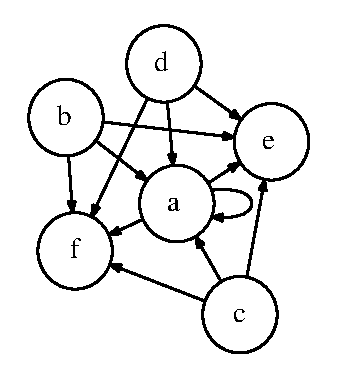
\includegraphics{images/non-reversible-reaction-example.dot.eps}
    \caption{Grafo ottenuto da una reazione non reversibile}
    \label{fig:non-reversible-reaction-mapping}
  \end{figure}
\item data una reazione reversibile $r$ tale che:
  \begin{displaymath}
    \begin{split} 
      reagenti(r) &= \{ r_{1}, \ldots, r_{n} \} \\
      prodotti(r) &= \{ p_{1}, \ldots, p_{m} \}
    \end{split}
  \end{displaymath}
  allora costruiremo il grafo che codifica la relazione $(reagenti(r)
  \times prodotti(r)) \cup (prodotti(r) \times reagenti(r))$. Ad
  esempio, con $reagenti(r) = \{ a, b, c, d \}$ e $prodotti(r) = \{a,
  e, f\}$ otteniamo il grafo riportato in Figura
  \ref{fig:reversible-reaction-mapping}.
  \begin{figure}
    \centering
    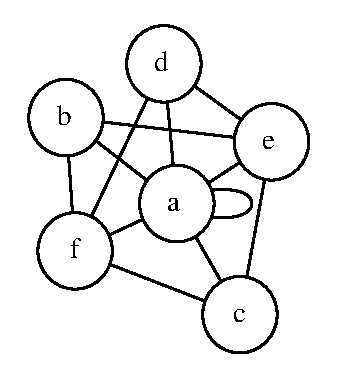
\includegraphics{images/reversible-reaction-example.dot.eps}
    \caption{Grafo ottenuto da una reazione reversibile}
    \label{fig:reversible-reaction-mapping}
  \end{figure}
\end{itemize}
Le regole descritte sopra pongono dei limiti sulle informazioni che si
codificano nel grafo finale. Per esempio tutti gli attributi delle
reazioni descritti in SBML vengono ignorati. Questo non rende
insufficiente la nostra rappresentazione in quanto miriamo alla
relazione di connessione estratta delle reazioni e non a loro
particolari propriet\`a.

Dobbiamo essere coscienti che applicando le precedenti regole facciamo
un passo di astrazione che comporta della perdita di precisione: nel
risultante grafo avremo codificato per ogni metabolito l'insieme di
metaboliti in cui questo pu\`o essere trasformato, a prescindere dalle
particolari reazioni che definiscono le trasformazioni.

\section{Riferimenti a lavori esistenti}
\label{section:existing-works}
Il lavoro esposto in \cite{large-scale-reconstruction} ha come
obiettivo lo studio di reti metaboliche per identificare quelli che
vengono chiamati nell'articolo originale \emph{seed sets}: questi
rappresentano degli insiemi di molecole che sono delle ``interfacce''
tra la rete metabolica e il contesto che la ospita. Una volta
identificati questi insiemi, si procede ad analizzarli e trarre
conclusioni di natura biologica.

Abbiamo citato questo lavoro in quanto condivide parte del processo di
astrazione della rete e l'applicazione di algoritmi con il presente
documento.
\\\\
Il nostro lavoro ha come obiettivo di essere d'ausilio al lavoro
esposto in \cite{tellingStories}, che studia una variante del problema
di enumerare tutti i sotto grafi aciclici di un grafo orientato,
aggiungendo il vincolo che solo un determinato sottoinsieme
$\mathbb{B}$ di vertici possono avere il ruolo di sorgente o di pozzo
nei \emph{DAG} enumerati. Ogni \emph{DAG} che soddisfa tale condizione
\`e chiamato \emph{storia} e si vuole ``raccontare'' tutte le
possibili storie dato un grafo orientato e l'insieme
$\mathbb{B}$. Ricordiamo che un \emph{DAG} \`e un grafo orientato che
non contiene cicli.

\section{Nostri obiettivi}
Il concetto catturato dall'insieme $\mathbb{B}$, introdotto nella
precedente sezione, \`e quello di definire il ruolo che alcuni vertici
``interpreteranno'' nella \emph{storia} (se $v \in \mathbb{B}$ allora
$v$ avr\`a il ruolo di \emph{sorgente} o \emph{pozzo}, altrimenti il
ruolo di \emph{intermedio}).

Attualmente l'insieme $\mathbb{B}$ viene costruito in base a
osservazioni e studi \emph{empirici}, ed \`e costituito dall'insieme
di metaboliti che hanno particolari propriet\`a in determinate
condizioni.  Ci chiediamo se \`e possibile identificare l'insieme
$\mathbb{B}$ in modo automatico per analizzare la rete metabolica
utilizzando gli algoritmi esposti in \cite{tellingStories}.
\\\\
Per rispondere a tale domanda abbiamo deciso di analizzare la
connettivit\`a del grafo in input, ricercando le sue componenti
fortemente connesse. Questa idea si basa sulle seguenti motivazioni:
\begin{itemize}
\item \`e difficile cercare di assegnare il ruolo ad ogni vertice
  studiando l'istanza completa del grafo in input, in quanto astrarre
  una rete metabolica comporta grafi con molti vertici e numerosi
  archi ed, inoltre, possono esistere (con molta frequenza) cicli che
  portano solo ridondanza e complessit\`a, che quindi possiamo
  escludere in quanto non aggiungono informazioni.

  Identificando invece la decomposizione in componenti fortemente
  connesse, \`e possibile astrarre dai cicli ed identificare classi di
  metaboliti equivalenti che possono essere visti come uno solo;
\item come vedremo nella Sezione \ref{subsection:some-definitions},
  ogni componente fortemente connessa \`e una classe di equivalenza
  della relazione di connessione forte. 

  Ci\`o significa che due metaboliti appartenenti alla stessa
  componente fortemente connessa possono essere ottenuti l'uno
  dall'altro, attraverso una catena di reazioni nella rete metabolica
  che stiamo analizzando. Possiamo quindi associare a questi
  metaboliti lo stesso ruolo che viene associato alla componente che
  li contiene;
\item il ``meta grafo'' che ha come vertici le componenti fortemente
  connesse e come archi gli archi che collegano metaboliti contenuti
  in componenti diverse (evitando duplicazioni), permette di assegnare
  alle componenti un ruolo. Se una componente \`e \emph{sorgente} o
  \emph{pozzo} nel meta grafo allora possiamo inserire i vertici che
  la compongono nell'insieme $\mathbb{B}$.
\end{itemize}
Utilizzando quanto detto sopra procederemo ad applicare al grafo in
input l'algoritmo di Tarjan (in realt\`a la variante descritta nella
Sezione \ref{subsection:crescenzi-gambosi-grossi}), determineremo il
ruolo delle componenti e, di conseguenza, sar\`a possibile assegnare
un ruolo anche ai vertici.
\\\\
Per automatizzare tutte le idee esposte nei paragrafi precedenti
abbiamo prodotto una libreria Java nella quale vengono implementati i
concetti esposti nel Capitolo
\ref{chapter:theoretical-background}. Questa libreria non \`e
orientata ad essere utilizzata come un programma a se stante, bens\`i
mira ad un utilizzo programmatico ed estendibile. Per questo motivo
abbiamo ritenuto opportuno riportare nella Sezione
\ref{section:packages-descriptions} una descrizione di ogni
\emph{pacchetto} in modo da favorirne la comprensione e l'utilizzo.

Nella libreria \`e presente anche una maschera realizzata utilizzando
il framework \emph{SWING} per la renderizzazione di un particolare
insieme di risultati, relativi alla composizione delle componenti
fortemente connesse: questo \`e l'unico oggetto che non \`e possibile
utilizzare programmaticamente.

\section{Sinopsi}
In questa sezione elenchiamo i capitoli in cui questo documento \`e
suddiviso e, per ognuno di essi, daremo una breve descrizione del
contenuto.

Questo capitolo contiene un'introduzione al lavoro svolto.

Il Capitolo \ref{chapter:theoretical-background} modella da un punto
di vista teorico i concetti e gli algoritmi alla base delle
implementazioni, in particolare cosa significa visitare un grafo,
approfondiremo la strategia \emph{Depth First} e studieremo tre
algoritmi per la ricerca delle componenti fortemente connesse.

Il Capitolo \ref{chapter:study} formalizza gli obiettivi che vogliamo
raggiungere con lo sviluppo della libreria Java. Vengono proposti i
casi d'uso che abbiamo implementato e, per ognuno di essi, vengono
riportati degli esempi del ``prodotto finito'' in modo da visualizzare
i risultati se non si \`e avuto modo di utilizzare la
libreria. Inoltre si analizza l'architettura che caratterizza l'intera
implementazione.

Il Capitolo \ref{chapter:conclusions} termina il lavoro esponendo i
risultati ottenuti ed elencando una lista di sviluppi futuri del
progetto.

Il Capitolo \ref{chapter:implementation} affronta tutte le questioni
inerenti alla fase di implementazione. Si discute la metodologia di
sviluppo utilizzata ed i \emph{pacchetti} che compongono il progetto.


\section{Strumenti utilizzati}
\label{section:used-tools}
Per lo sviluppo di questo progetto sono stati utilizzati i seguenti
strumenti:
\begin{itemize}
\item per la stesura di questo documento \`e stato usato il motore di
  formattazione \TeX, utilizzando \emph{Emacs} come editor dei file
  sorgenti, installando la \emph{major mode AucTex};
\item l'implementazione della libreria Java \`e stata sviluppata
  completamente con \emph{Eclipse} versione \emph{Indigo}. La JVM
  utilizzata per lo sviluppo \`e quella fornita da \emph{openjdk-6
    (versione 24)};
\item i sorgenti, sia dell'elaborato testuale sia
  dell'implementazione, sono stati versionati utilizzando il sistema
  \emph{Git}. Abbiamo utilizzato \emph{Github} come fornitore del
  servizio. I sorgenti di questo documento possono essere scaricati
  dall'URL:\\
  \href{https://github.com/massimo-nocentini/my-undergraduate-thesis}{
    https://github.com/massimo-nocentini/my-undergraduate-thesis}\\
  mentre i sorgenti dell'implementazione Java dall'URL:\\
  \href{https://github.com/massimo-nocentini/my-undergraduatethesis-java}{
    https://github.com/massimo-nocentini/my-undergraduatethesis-java}
\end{itemize}